\documentclass{beamer}
\setbeameroption{show notes} % un-comment to see the notes
\setbeamertemplate{itemize items}[triangle]

\mode<presentation>{ 
  %\usetheme{AnnArbor}
  %\usetheme{Antibes}
  %\usetheme{Bergen}
  %\usetheme{Berkeley}
  %\usetheme{Berlin}
  %\usetheme{Boadilla}
  %\usetheme{boxes}
  %\usetheme{CambridgeUS}
  %\usetheme{Copenhagen}
  %\usetheme{Darmstadt}
  %\usetheme{default}
  %\usetheme{Frankfurt}
  %\usetheme{Goettingen}
  %\usetheme{Hannover}
  %\usetheme{Ilmenau}
  %\usetheme{JuanLesPins}
  %\usetheme{Luebeck}
  \usetheme{Madrid}
  %\usetheme{Malmoe}
  %\usetheme{Marburg}
  %\usetheme{Montpellier}
  %\usetheme{PaloAlto}
  %\usetheme{Pittsburgh}
  %\usetheme{Rochester}
  %\usetheme{Singapore}
  %\usetheme{Szeged}
  %\usetheme{Warsaw}
    
  \usecolortheme{default}
  %\usecolortheme{albatross}
  %\usecolortheme{beaver}
  %\usecolortheme{beetle}
  %\usecolortheme{crane}
  %\usecolortheme{dolphin}
  %\usecolortheme{dove}
  %\usecolortheme{fly}
  %\usecolortheme{lily}
  %\usecolortheme{orchid}
  %\usecolortheme{rose}
  %\usecolortheme{seagull}
  %\usecolortheme{seahorse}
  %\usecolortheme{whale}
  %\usecolortheme{wolverine}
  
  \usefonttheme{default}  % or try serif, structurebold, ...
  \setbeamertemplate{navigation symbols}{}
}

%\usepackage[spanish, es-tabla]{babel} % provide language hyphenation
\usepackage[utf8]{inputenc} % use UTF8 encoding

\usepackage{fancyhdr} % allows fancy headers
\usepackage{xcolor} % define colors

\usepackage{amsmath} % mathematical equations
\usepackage{amssymb} % add maths symbols
\usepackage{mathtools} % more maths symbols

\usepackage{graphicx} % add figures
\usepackage{caption} % caption customization
\usepackage{subcaption} % subfigures caption customization
\usepackage{geometry} % page layout modification
\usepackage{tikz} % tikz figures

%\usepackage{enumitem} % enumerate customization
\usepackage{glossaries} % add glossaries
\usepackage{listings} % code listing
%\usepackage{algorithm}
%\usepackage{algpseudocode}
\usepackage[ruled, linesnumbered]{algorithm2e}

\usepackage{cite} % citing
\usepackage{hyperref} % produces hypertext links
\usepackage{verbatim} % multiline comments

\usepackage{multirow} % more table options (e.g. multitables)
\usepackage{booktabs} % even more table options

\usepackage{todonotes} % todo notes

\newcommand{\Nn}{\mathcal{N}}
\newcommand{\Cc}{\mathcal{C}}
\newcommand{\Ee}{\mathcal{E}}
\newcommand{\bs}{\boldsymbol}
\newcommand{\defi}{\vcentcolon=}
\renewcommand{\it}{\textit}

\usepackage{lmodern}

\title[GraphSLAM Implementation]{Thesis Defense}
\subtitle{GraphSLAM Algorithm Implementation for Solving SLAM}
\date{\vspace{0em}\today}

\begin{document}
	
\begin{frame}
\author{
\hspace{-4em}
\begin{tabular}{rl} 
 \textbf{Author:}  & Franco Curotto \\
 \textbf{Thesis Adviser:} & Martin Adams \\ 
 \textbf{Commission Members:} & Marcos Orchard \\
 & Jorge Silva
\end{tabular}
\vspace{0em}
}
    
\includegraphics[width=0.4\textwidth]{img/fcfm_die.pdf}
    \titlepage
\end{frame}

\note[itemize]{
\item You may be wondering what GraphSLAM and SLAM
\item My work is ... in the field of robotics
}

\begin{frame}{Motivation}
\begin{columns}
\column{0.5\textwidth}
\centering
\textbf{Robots Before}\\
\vspace{1em}
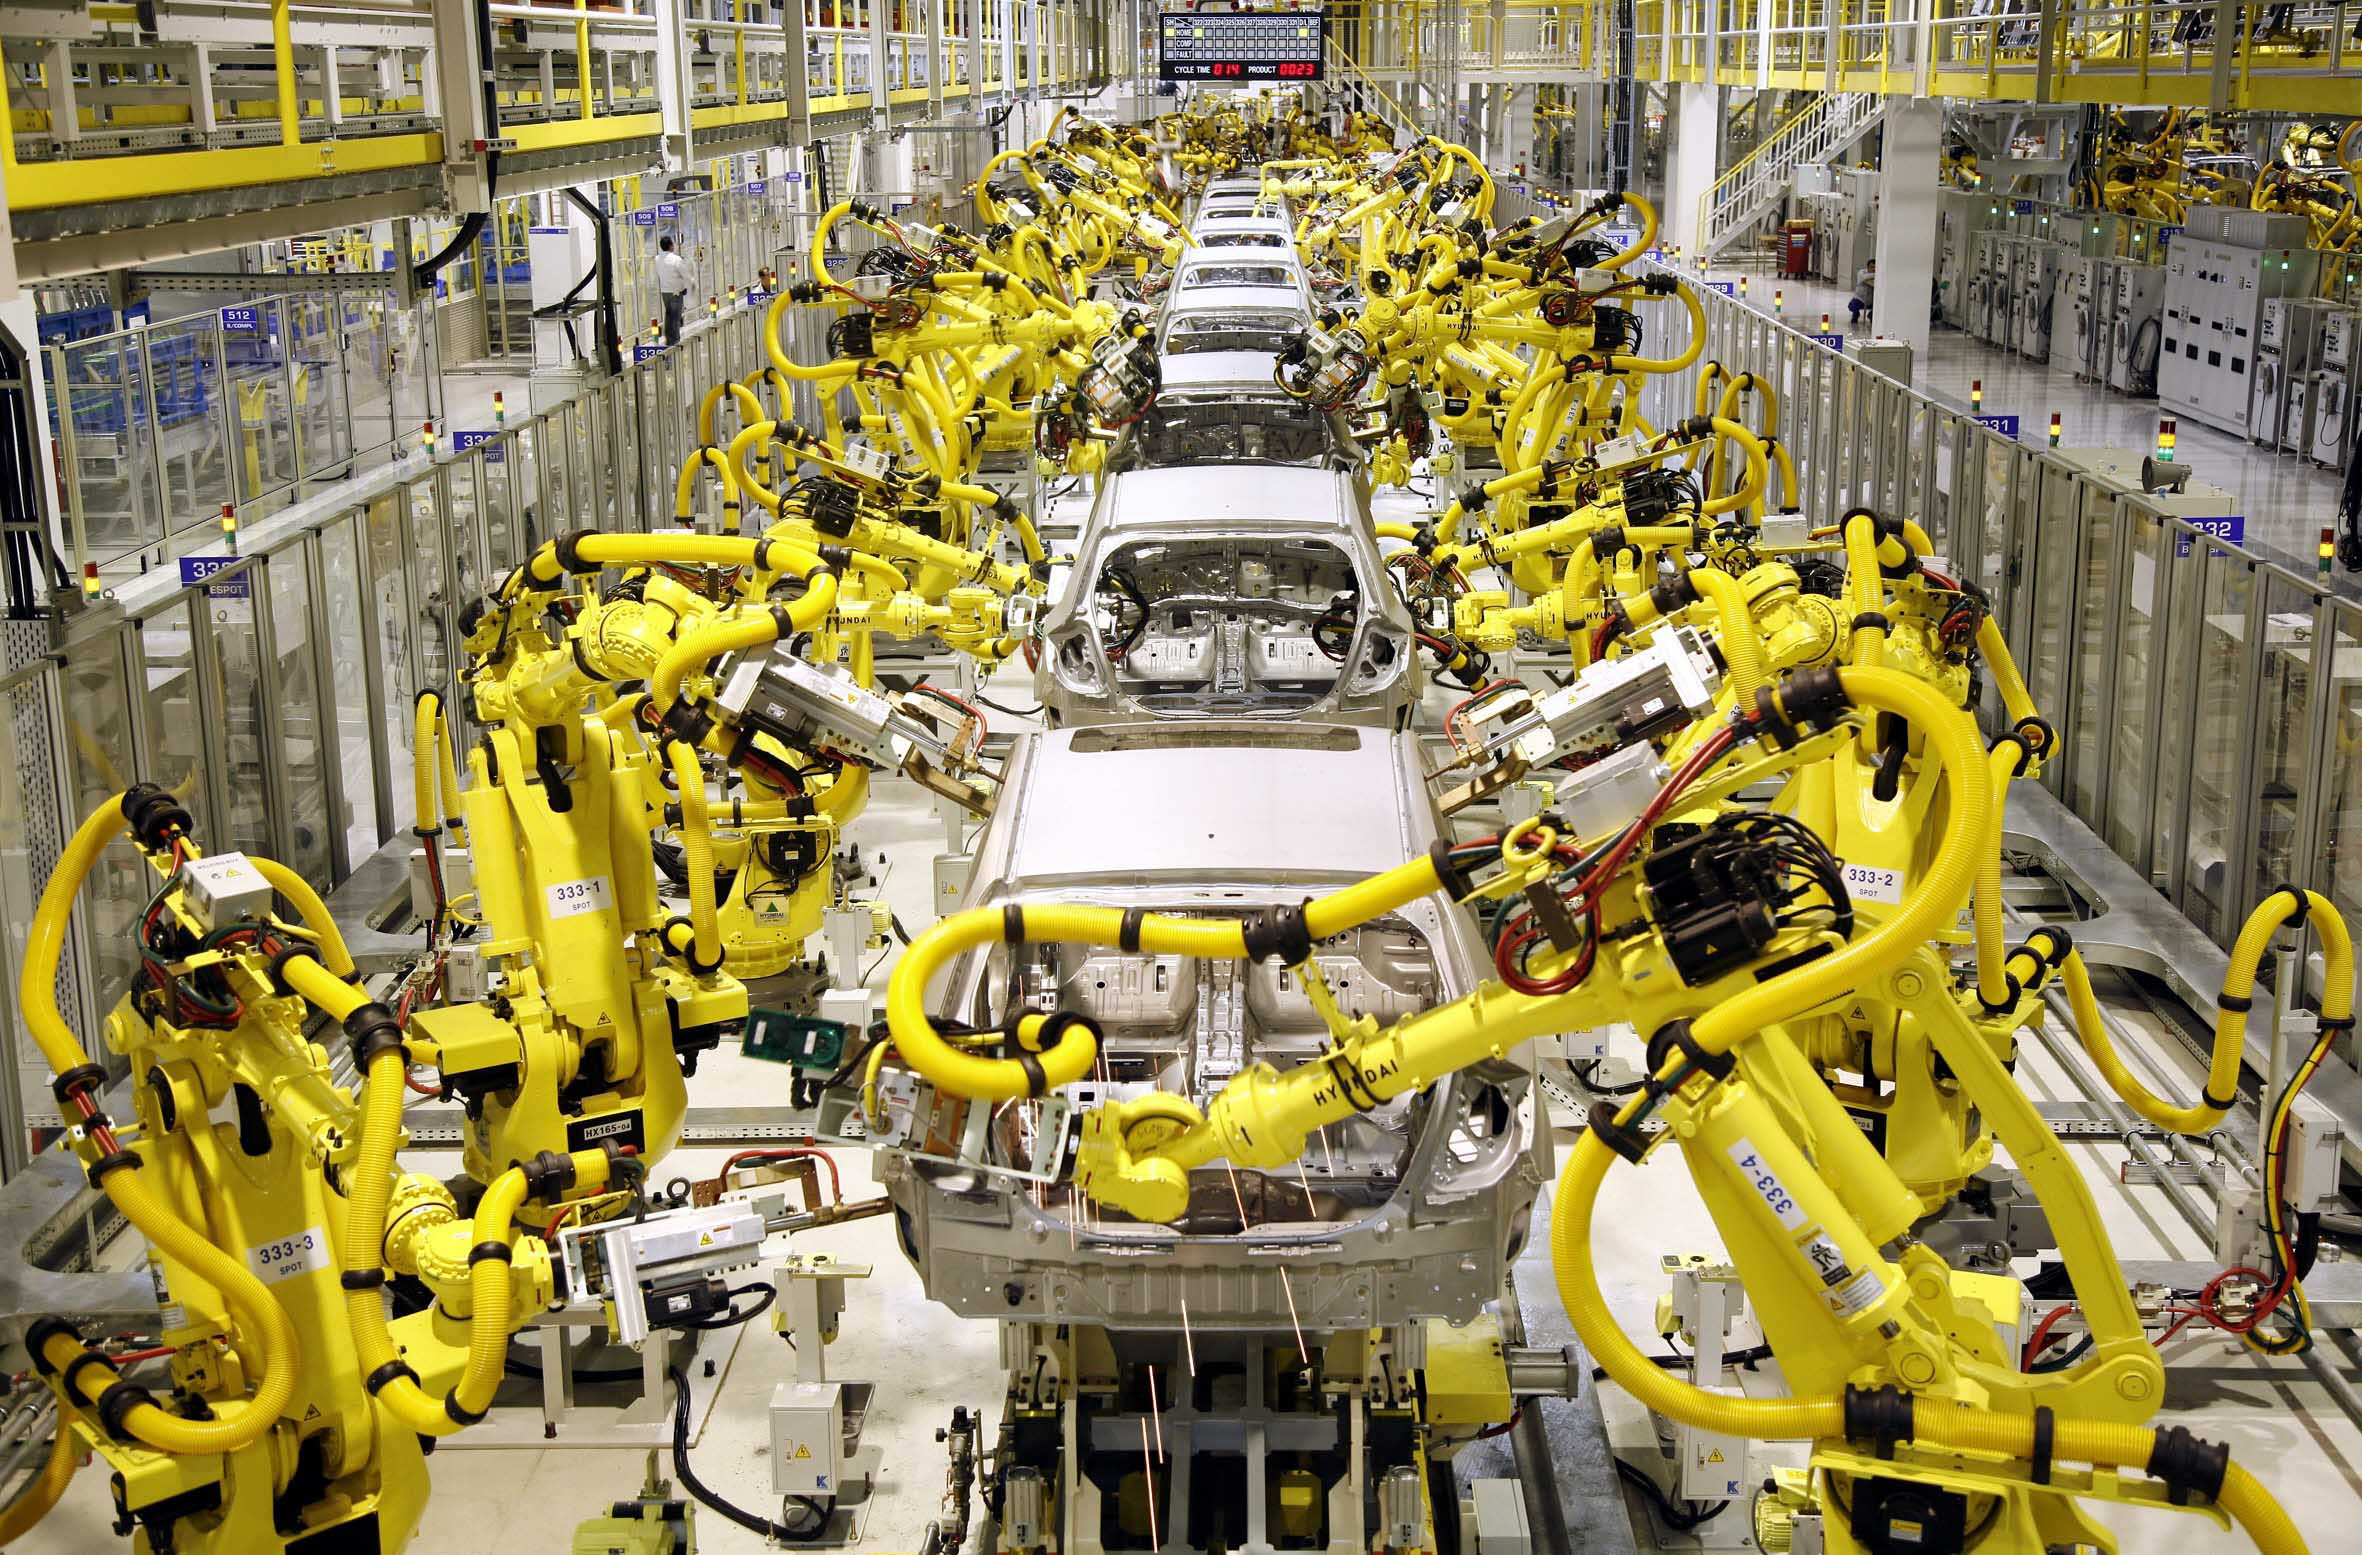
\includegraphics[width=0.8\textwidth]{img/assembly.jpg}\\
\vspace{1em}
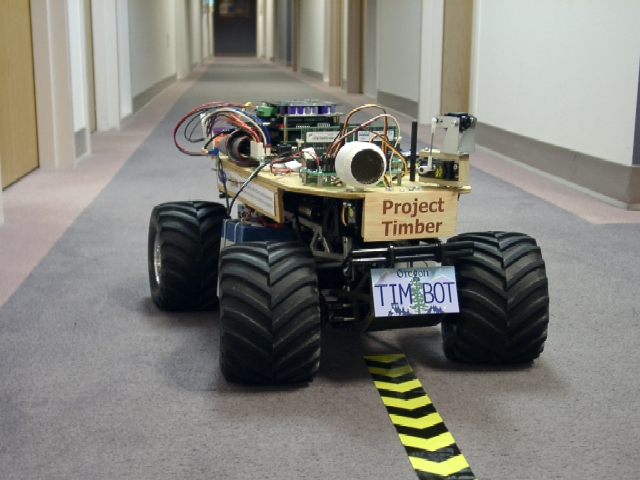
\includegraphics[width=0.8\textwidth]{img/timbot.jpg}
\column{0.5\textwidth}
\centering
\textbf{Robots Now}\\
\vspace{1em}
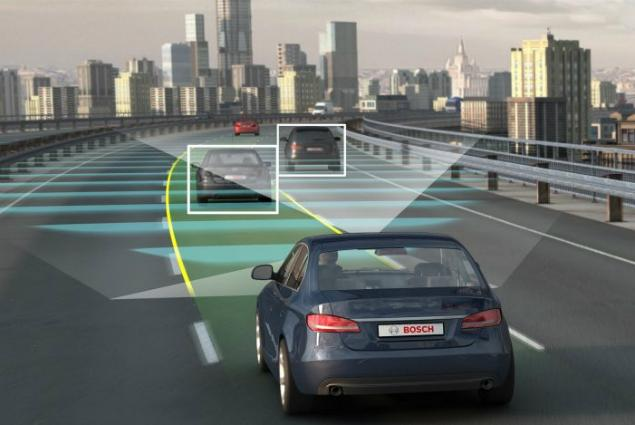
\includegraphics[width=0.8\textwidth]{img/selfdriving.jpg}\\
\vspace{1em}
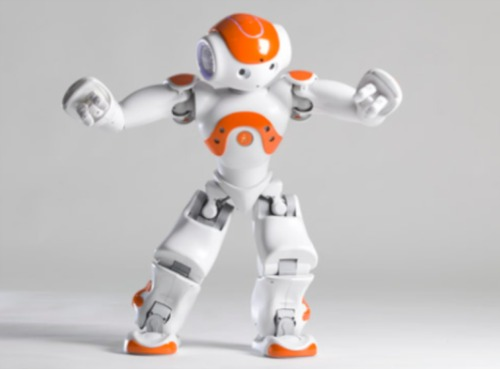
\includegraphics[width=0.8\textwidth]{img/nao.jpg}
\end{columns}
\end{frame}

\note[itemize]{
\item Robots in the past were restricted to do simple, repetitive tasks, and were either stationary [reference photo], or had limited mobility, usually by following a reference [reference photo]. 
\item Robots nowadays need to be much more versatile, autonomous and robust [reference photos].
\item In particular robots must be able to move freely in an open environment.
}

\begin{frame}{Motivation}
\begin{columns}
\column{0.5\textwidth}
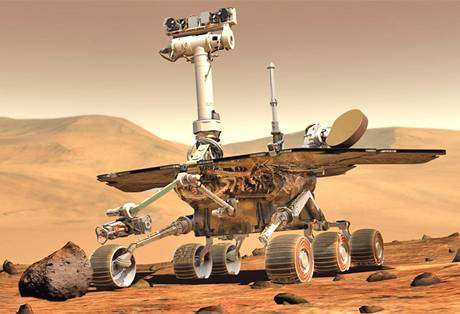
\includegraphics[width=0.8\textwidth]{img/mars-rover.jpg}\\
\column{0.5\textwidth}
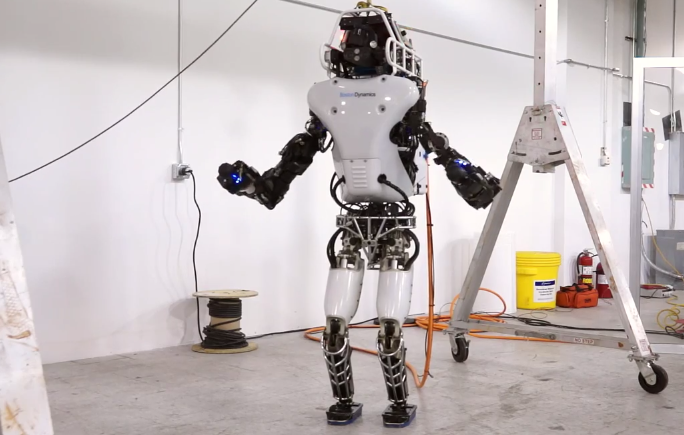
\includegraphics[width=0.8\textwidth]{img/atlas2.png}\\
\end{columns}
\vspace{1em}
\begin{block}{Mobile Robots}
\begin{itemize}
\item \textbf{Move} around known environments without getting lost.
\item \textbf{Explore} new environments, and ``remember'' them. 
\item \textbf{React} to unexpected changes.
\item  Perform their tasks in \textbf{suboptimal conditions}. 
\end{itemize}
\end{block}
\end{frame}

\note[itemize]{
\item A robot must be able to identify where in the scenario he is standing on.
\item For example if you buy a robot for your house, he never has seen your house before, so he must be able to explore it and remember it for later use.
\item For example when the environment changes, or when there is something moving on the room.
}

\begin{frame}{SLAM}
\begin{block}{Simultaneous Localization And Mapping (SLAM)}
\begin{center}
\textit{
The problem were an agent must simultaneously estimate its current position (localization), and construct a map of its environment (mapping).}
\end{center}
\end{block}
\begin{block}{Odometry and Measurements}
Sensors can be used to:
\begin{itemize}
\item Keep track of the robot movements (odometry)
\item Sense nearby objects positions (measurements)
\end{itemize}
Sensors are noisy. We can use probabilistic tool to improve sensors estimates.
\end{block}
\begin{columns}
\column{0.5\textwidth}
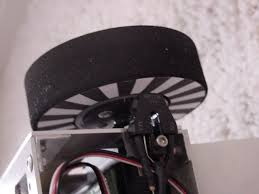
\includegraphics[width=0.6\textwidth]{img/encoders.jpg}
\centering
\column{0.5\textwidth}
\centering
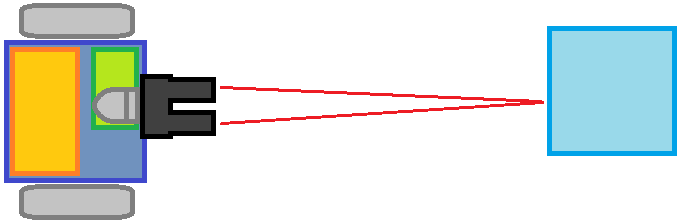
\includegraphics[width=0.8\textwidth]{img/laser.png}
\end{columns}
\end{frame}

\begin{frame}{GraphSLAM}
GraphSLAM description
\end{frame}

\begin{frame}{Implementation}
Implementation details
\end{frame}

\begin{frame}{Results}
\end{frame}

\begin{frame}{Conclusions}
\end{frame}

\begin{frame}
\author{
\hspace{-4em}
\begin{tabular}{rl} 
 \textbf{Author:}  & Franco Curotto \\
 \textbf{Thesis Adviser:} & Martin Adams \\ 
 \textbf{Commission Members:} & Marcos Orchard \\
 & Jorge Silva
\end{tabular}
\vspace{0em}
}
    
\includegraphics[width=0.4\textwidth]{img/fcfm_die.pdf}
    \titlepage
\end{frame}

\end{document}

